\documentclass[tikz,border=8pt]{standalone}
\usepackage{amsmath,amssymb}
\usetikzlibrary{arrows.meta,automata,positioning,quotes}
\begin{document}
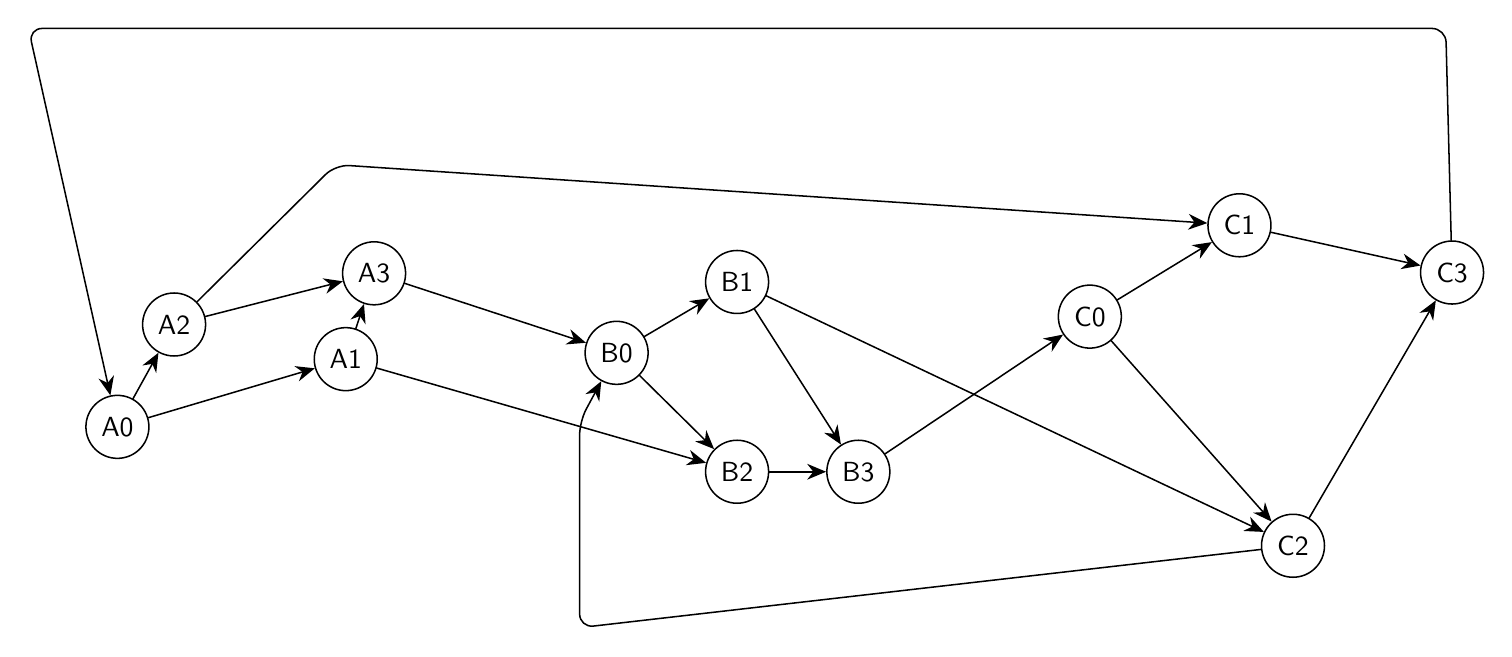
\begin{tikzpicture}[x=1cm,y=1cm]
\tikzset{
  graphnode/.style={circle,draw=black,line width=0.55pt,minimum size=8mm,inner sep=1pt,font=\sffamily},
  graphedge/.style={draw=black,line width=0.55pt,line cap=round,line join=round},
  directed/.style={graphedge,-{Stealth[length=2.4mm,width=2.0mm]}},
  undirected/.style={graphedge}
}
\node[graphnode] (n_A0) at (-7.87,-1.31) {A0};
\node[graphnode] (n_A1) at (-4.97,-0.45) {A1};
\node[graphnode] (n_A2) at (-7.15,-0.01) {A2};
\node[graphnode] (n_A3) at (-4.61,0.64) {A3};
\node[graphnode] (n_B0) at (-1.53,-0.37) {B0};
\node[graphnode] (n_B1) at (0.00,0.53) {B1};
\node[graphnode] (n_B2) at (0.00,-1.88) {B2};
\node[graphnode] (n_B3) at (1.54,-1.88) {B3};
\node[graphnode] (n_C0) at (4.48,0.09) {C0};
\node[graphnode] (n_C1) at (6.38,1.25) {C1};
\node[graphnode] (n_C2) at (7.06,-2.82) {C2};
\node[graphnode] (n_C3) at (9.08,0.65) {C3};
\draw[directed] (n_A0) -- (n_A1);
\draw[directed] (n_A0) -- (n_A2);
\draw[directed] (n_A1) -- (n_A3);
\draw[directed] (n_A2) -- (n_A3);
\draw[directed] (n_B0) -- (n_B1);
\draw[directed] (n_B0) -- (n_B2);
\draw[directed] (n_B1) -- (n_B3);
\draw[directed] (n_B2) -- (n_B3);
\draw[directed] (n_C0) -- (n_C1);
\draw[directed] (n_C0) -- (n_C2);
\draw[directed] (n_C1) -- (n_C3);
\draw[directed] (n_C2) -- (n_C3);
\draw[directed] (n_A3) -- (n_B0);
\draw[directed] (n_B3) -- (n_C0);
\draw[directed] (n_A1) -- (n_B2);
\draw[directed,rounded corners=5pt] (n_A2) -- (-5.10,2.02) -- (n_C1);
\draw[directed] (n_B1) -- (n_C2);
\draw[directed,rounded corners=5pt] (n_C3) -- (9.00,3.75) -- (-9.00,3.75) -- (n_A0);
\draw[directed,rounded corners=5pt] (n_C2) -- (-2.00,-3.86) -- (-2.00,-1.24) -- (n_B0);
\end{tikzpicture}
\end{document}
